\documentclass[12pt, twoside]{article}
\usepackage[letterpaper, margin=1in, headsep=0.5in]{geometry}
\usepackage[english]{babel}
\usepackage[utf8]{inputenc}
\usepackage{amsmath}
\usepackage{amsfonts}
\usepackage{amssymb}
\usepackage{tikz}
\usetikzlibrary{quotes, angles}
\usepackage{graphicx}
\usepackage{enumitem}
\usepackage{multicol}
\usepackage{hyperref}

\newif\ifmeta
\metatrue %print standards and topics tags

\title{IB Mathematics}
\author{Chris Huson}
\date{March 2022}

\usepackage{fancyhdr}
\pagestyle{fancy}
\fancyhf{}
\renewcommand{\headrulewidth}{0pt} % disable the underline of the header
\raggedbottom


\fancyhead[LE]{\thepage}
\fancyhead[RO]{\thepage \\ Name: \hspace{4cm} \,\\}
\fancyhead[LO]{BECA / IB Math 5 Exponential functions \\* 9 March 2022}

\begin{document}
\subsubsection*{5.10 Quiz: Exponential functions (DRAFT)}
\emph{Round all currency amounts to the nearest hundredth.}
\begin{enumerate}
\item Frank puts \$2,000 into an investment account with an annual interest rate of 3.00\%. Find the balance after one year. \vspace{1.5cm}

\item Allen invests \$87,500 in an account with an annual interest rate of 2.85\%. Find the balance after 4 years. \vspace{1.5cm}

\item Sharia puts \$30,000 into an investment account with an annual interest rate of 4.25\%. Find the number of years required for the balance to reach \$38,510.37. \vspace{2cm}

\item A bond with a three year maturity and principal amount of \$10,000 compounds monthly with an annual interest rate of 3.00\%.
\begin{enumerate}[itemsep=0.5cm]
    \item How many compounding periods are there per year? \\[0.25cm]
    $k=$
    \item Find the final balance of principal and interest after three years.
\end{enumerate} \vspace{1.5cm}

\item Lily invested SGD 2000 (Singapore dollars) in an account that pays 1.85\% interest per year compounded monthly. (show your working with a labeled sketch using the axes)
\begin{multicols}{2}
    \begin{enumerate}[itemsep=1cm]
        \item Find how much Xi had in the account after 3 years.
        \item Find the number of years until he had SGD 3400 in the account.
    \end{enumerate} \vspace{0.5cm}
    \begin{flushright}
    \begin{tikzpicture}
        \draw [thick, ->] (0,0)--(6,0);
        \draw [thick, ->] (0,0)--(0,6);
    \end{tikzpicture}
    \end{flushright}
\end{multicols}


\newpage
\item The graph shows the exponential function $\displaystyle FV=1200 \times \left( 1+\frac{3.00}{100} \right)^t$ representing the balance of an investment account earning a fixed rate of interest over $t$ in years.
\begin{multicols}{2}
    \begin{enumerate}[itemsep=1cm]
        \item Write down the initial deposit in the account.
        \item Write down the annual interest rate.
        \item How much will the account hold at the end of ten years, to the nearest hundred dollars?
        \item When will the balance be \$1600, to the nearest year?
    \end{enumerate}\vspace{1cm}
    \begin{center}
    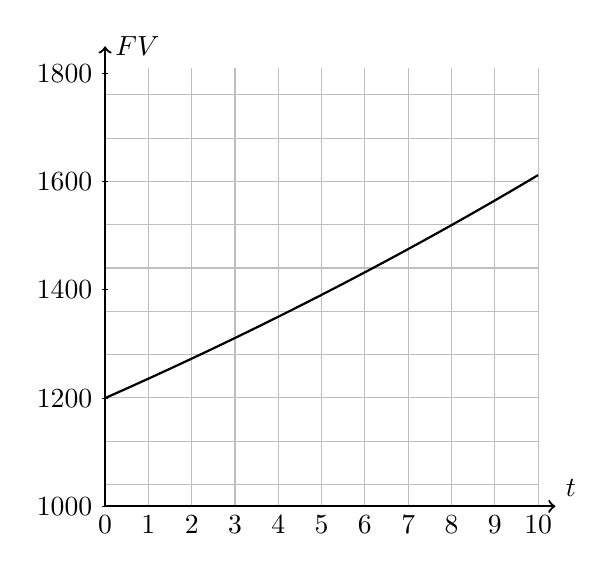
\begin{tikzpicture}[x=1cm, y=0.0125cm, scale=0.55]
        \draw [thin, color=lightgray, xstep=1.0cm,ystep=1.0cm] (0,1000) grid (10,1810);
        \draw [thick, ->] (0,1000) -- (+10.4,1000) node [above right]{$t$};
        \draw [thick, ->] (0,1000) -- (0,1850) node [right]{$FV$};        \foreach \x in {0,1,...,10}
            \draw (\x cm,1000) -- (\x cm,1000) node[below] {$\x$};
        \foreach \y in {1000,1200,...,1800}
            \draw[shift={(0,\y)}] (2pt,0pt)--(-2pt,0pt) node[left]{$\y$};
        \draw [thick, smooth,domain=0.:10] plot(\x,{1200*(1.03^\x)});
    \end{tikzpicture}
    \end{center}
    \end{multicols}

\item The half life of radioactive iodine 131 is eight days. That is, one half of this isotope decays over this period of time. Given an intial amount of $I_{131}$ of $N_0$, use this formula for the amount remaining $N(t)$ as a function of time $t$ in days: \[\displaystyle N(t)=N_0 \times \left( \frac{1}{2} \right)^{t/8}\]  \vspace{0.25cm}
    \begin{multicols}{2}
        \begin{enumerate}[itemsep=0.5cm]
            \item How long does it take for half of a given amount of $I_{131}$ to decay?
            \item Find the fraction of iodine 131 that would remain after 30 days. \vspace{0.75cm}
            \item Find the time for 99 percent to decay.
        \end{enumerate} \vspace{0.5cm}
        \begin{center}
        \begin{tikzpicture}
            \draw [thick, ->] (0,0)--(5,0);
            \draw [thick, ->] (0,0)--(0,6);
        \end{tikzpicture}\\[0.5cm]
        Sketch a labeled graph as working.
        \end{center}
        
    \end{multicols}

\newpage
\item A fruit fly population doubles every 5 days. There are currently ten fruit flies in a laboratory container. With $t$ representing time, in days, then the population of flies can be modeled by \[\displaystyle P(t)=A \times b^{t/3}\]
    %Alg2 Regents Jan2017
    \begin{enumerate}[itemsep=0.75cm]
        \item Write down the value of $A$
        \item Write down the value of $b$
        \item About how many flies will there be in two weeks? \vspace{1.5cm}
        \item Find the time needed to reach a population of 160.
    \end{enumerate} \vspace{1.5cm}
    
\item Graph $\displaystyle f(t)=75,000 \left( 1-0.25 \right)^t$, representing the depreciation of an asset over $t$ years.
\begin{multicols}{2}
    \begin{enumerate}[itemsep=1.2cm]
        \item Write down the initial cost of the asset.
        \item Write down the percentage value lost each year.
        \item Find the value of the investment after one year.\vspace{1cm}
        \item Find the number of years to depreciate half of the value.
    \end{enumerate}
    \begin{center}
    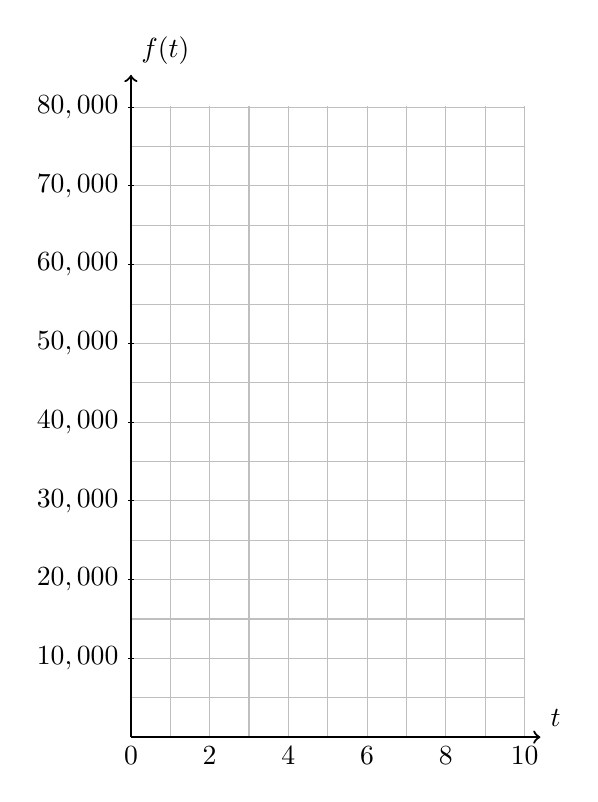
\begin{tikzpicture}[x=1cm, y=0.0002cm, scale=0.50]
        \draw [thin, color=lightgray,xstep=1.0cm,ystep=1cm](0,0) grid (10,81000);
        \draw [thick, ->] (0,0) -- (+10.4,0) node [above right]{$t$};
        \draw [thick, ->] (0,0) -- (0,85000) node [above right]{$f(t)$};        
        \foreach \x in {0,2,...,10}
            \draw (\x cm,0) -- (\x cm,0) node[below] {$\x$};
        \foreach \y in {1,2,...,8}
            \draw[shift={(0,2*\y cm)}] (2pt,0pt)--(-2pt,0pt) node[left]{$\y0,000$};
        %\draw [thick, smooth,domain=0:10] plot(\x,{1700*(1.095^\x)});
    \end{tikzpicture}
    \end{center}
    \end{multicols}

\newpage
\item The spread of a virus in the lungs is modeled by $\displaystyle y= 15 e^x$, with $x$ the time in hours. 
\begin{enumerate}[itemsep=1cm]
    \item Find the quantity of the meme after two hours.
    \item Find the number of hours for meme to spread to 33,000.
\end{enumerate} \vspace{2cm}

\item The temperature of hot ingot as it cools is modeled by the function 
    \[ T(x)=150e^{-0.07x}+45 \] where $T(x)$
    is the temperature in degrees Celsius and $x$ is the time in hours.
    \begin{enumerate}[itemsep=1cm]
        \item Write down the initial temperature at time zero.
        \item Find the temperature after 24 hours.
        \item Find the time to cool to $100^\circ$C.
        \item Graph the ingot's temperature. Label each of your answers with their values.
    \end{enumerate}
    \begin{center}
    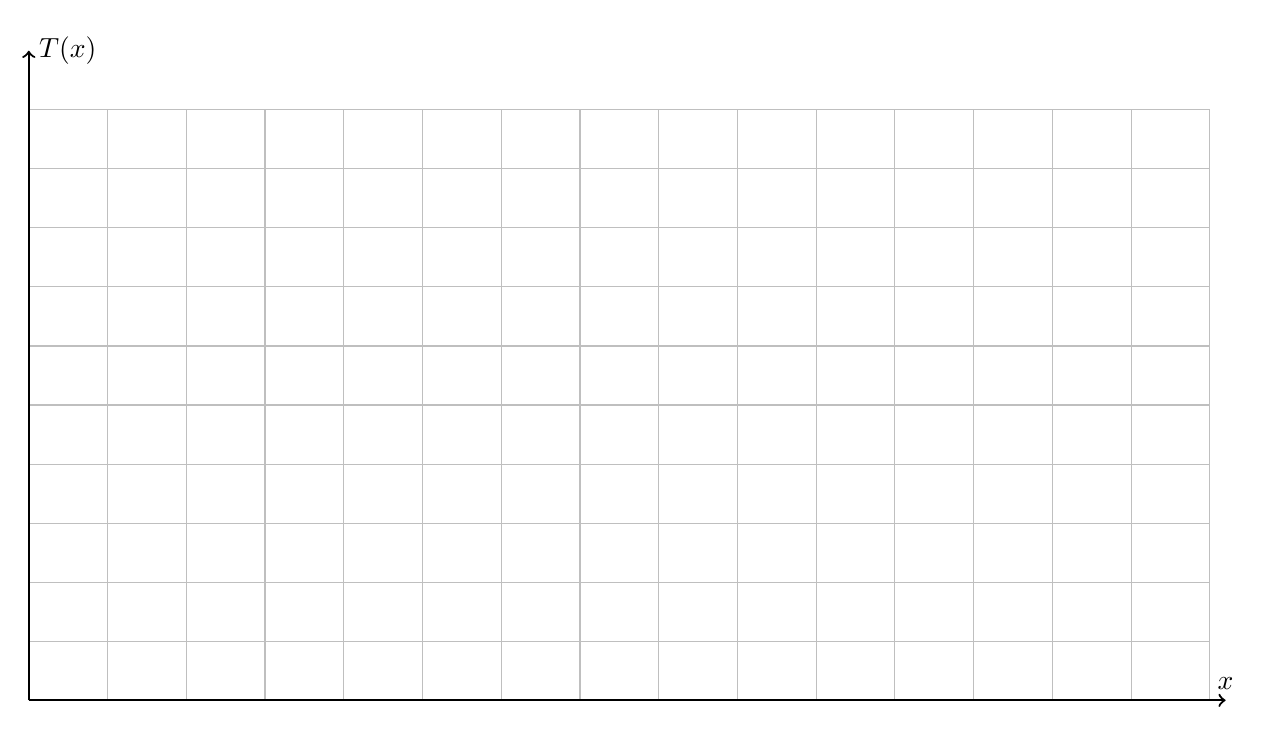
\begin{tikzpicture}[xscale= 0.2, yscale=0.015]
        \draw [thin,color=lightgray,xstep=5cm,ystep=50cm](0,0) grid (75,500);
        \draw [thick, ->] (0,0) -- (76,0) node [above] {$x$};
        \draw [thick, ->] (0,0) -- (0,550) node [right] {$T(x)$};
        %\foreach \x in {0,10,20,30,40,50,60}
            %\draw[shift={(\x,0)}] (0,10) -- (0,0) node[below]  {$\x$};
        %\foreach \y in {0,100,200,300,400,500}
            %\draw[shift={(0,\y)}] (0.5,0) -- (0,0) node[left]  {$\y$};
        %\draw plot[domain=0:60] (\x,{375*exp(-0.05*\x) +12.5});
    \end{tikzpicture}
    \end{center}

\end{enumerate}
\end{document}
